\subsection{完善simulink模型}

为了更加直观地感受车辆的操作响应,为simulink模型添加大地坐标系下X、Y坐标的计算。由书本图5-23及图5-24可清晰得知大地坐标系下车辆在
X轴和Y轴的速度分量与车辆的质心速度的关系分别为:
$$
\begin{cases}
    v_X = v_1 cos(\beta+\phi)\\
    v_Y = v1 sin(\beta+\phi)
\end{cases}
$$
式中$\beta$为质心侧偏角,可以由$arctan(v/u)$获得;$\phi$为车辆横摆角,可以通过横摆角速度积分获得。
完善后的simulink模型如下图所示:

\begin{figure}[h]
    \centering
    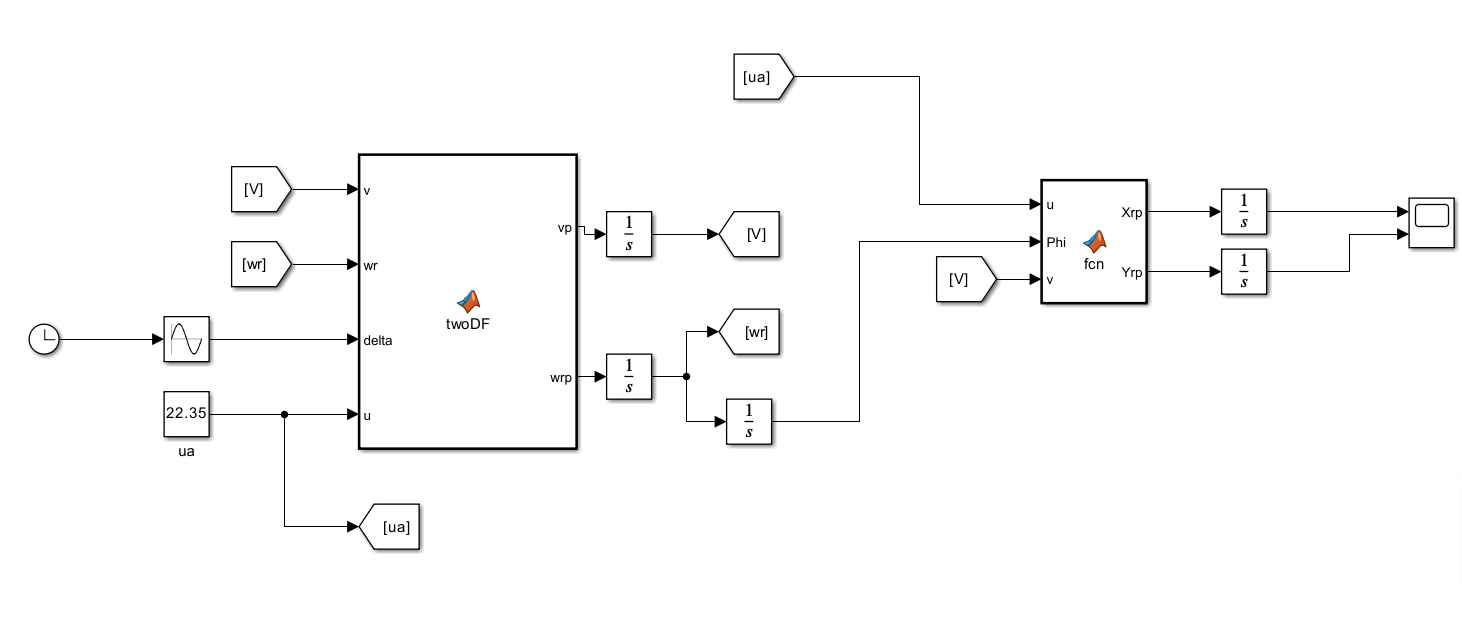
\includegraphics[width=10cm]{figure/final.png}
    \caption{带路径计算的simulink模型}
    \label{simulinkFinal}
\end{figure}

设定前轮转角在-30°-30°范围内以正弦规律转动,得到的车辆路径如图5所示:

\begin{figure}[htbp]
    \centering
    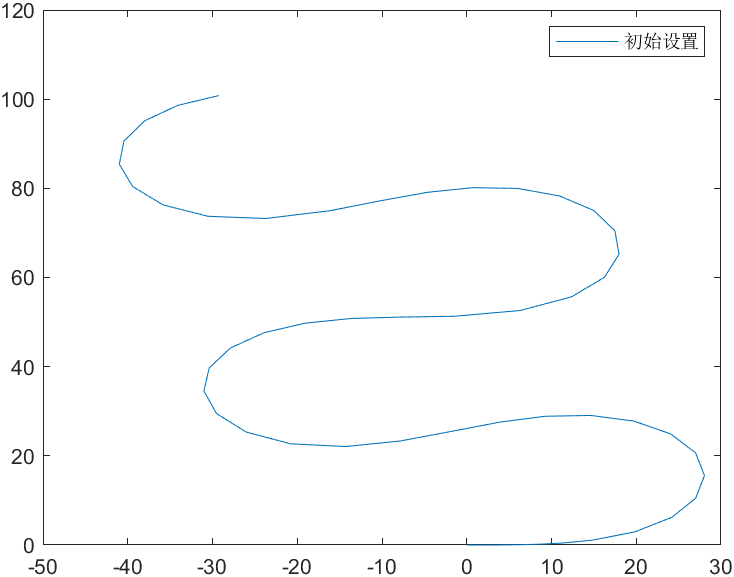
\includegraphics[width=5.5cm]{figure/origin.png}
    \caption{正弦波输入的车辆路径}
    \label{originpath}
\end{figure}

\subsection{改变车速}
设置车速分别为$10m/s,20m/s,30m/s$,运行时间为50s,车辆路径如图6所示:
\begin{figure}[htbp]
    \centering
    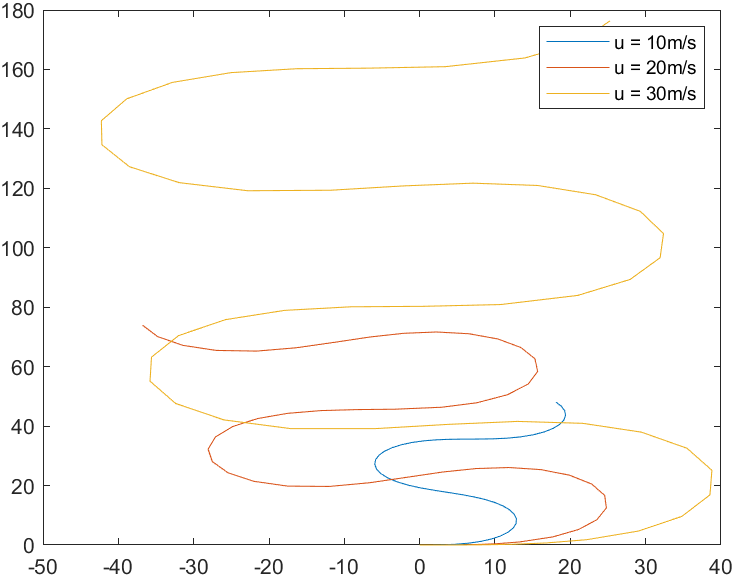
\includegraphics[width=5.5cm]{figure/velocity.png}
    \caption{不同车速下的车辆路径}
    \label{velocity}
\end{figure}

\subsection{改变车辆质量及转动惯量}
设置质量m分别为$1000kg,1818.2kg,2000kg$,转动惯量在保持$m=1818.2kg$时改变为$3000,4500kg\cdotm^2$时,车辆路径如图7所示:
\begin{figure}[htbp]
    \centering
    \subfigure[不同质量下的车辆路径]{
        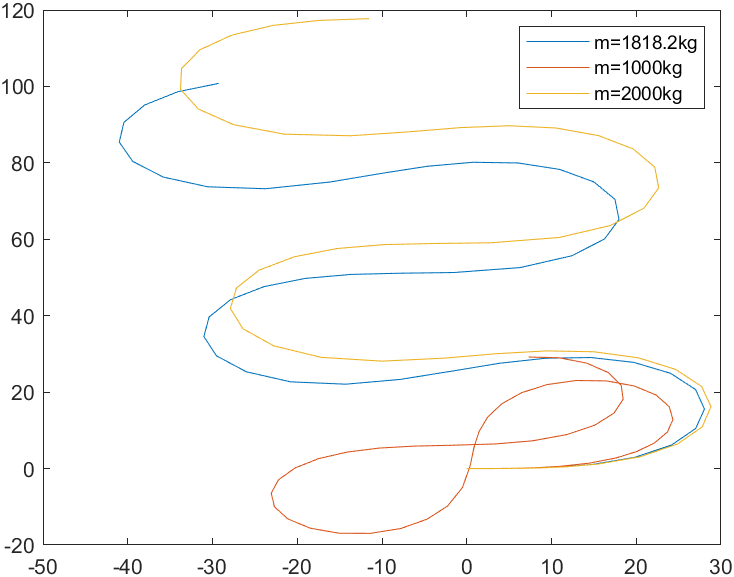
\includegraphics[width=5.5cm]{figure/mass.png}
    }
    \subfigure[不同转动惯量下的车辆路径]{
        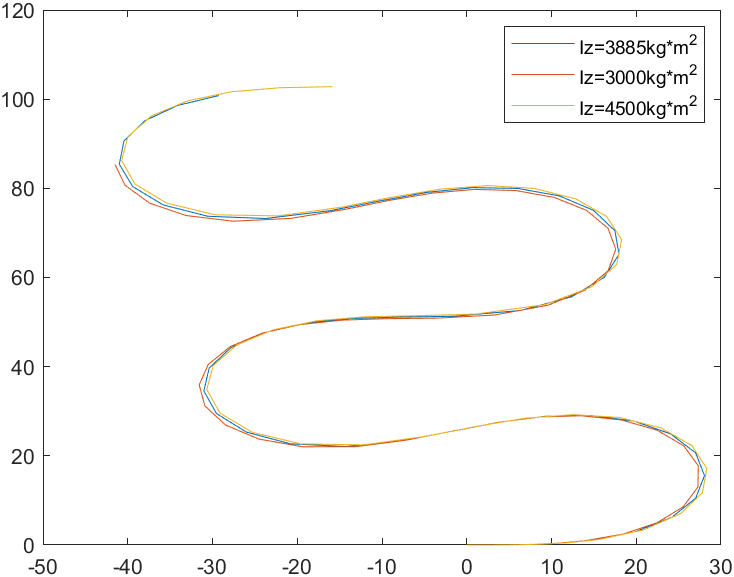
\includegraphics[width=5.5cm]{figure/Iz.png}
    }
    \caption{不同质量、转动惯量下的车辆路径}
    \label{massIz}
\end{figure}

可见质量会影响车辆的操作稳定性,而转动惯量的影响并不明显,主要原因是此时仅仅改变了车辆的转动惯量,事实上转动惯量改变时车辆的其他参数也会发生变化,因此此时研究的转动惯量对车辆操作响应的影响意义不大。

\subsection{改变车辆前轴后轴长度分配以及侧偏刚度}
使车辆前轴长于后轴,得到的车辆路径如图8(a)所示。
\begin{figure}[htbp]
    \centering
    \subfigure[不同前后轴长度分配下的车辆路径]{
        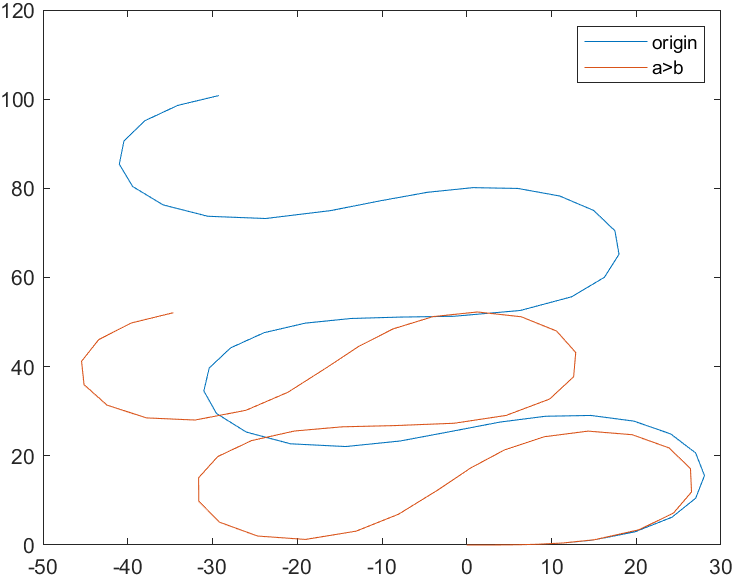
\includegraphics[width=5.5cm]{figure/length.png}
    }
    \subfigure[不同前后侧偏刚度下的车辆路径]{
        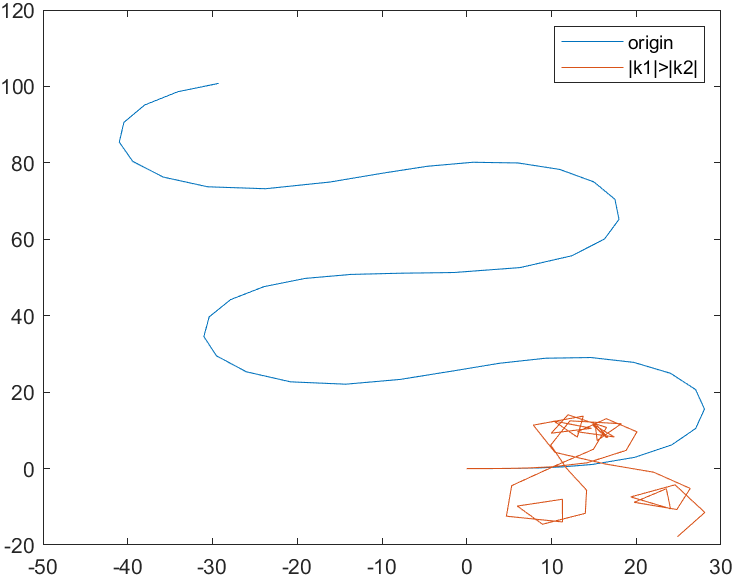
\includegraphics[width=5.5cm]{figure/k.png}
    }
\end{figure}

同理使前轮侧偏刚度的绝对值大于后轮侧偏刚度的绝对值,得到车辆路径如图8(b)所示。可见,当车辆前轴长度大于后轴或者前轮侧偏刚度大于后轮时,都会使车辆趋于过度转向,使操作响应变得不稳定。

